% !TEX root = ../main.tex
%==========================================%

\section{Introduction}\label{sec:Intro}

The first wave of cryptocurrencies, starting in the 1980s, attempted to provide a digitization of government-issued currency (or `fiat currency' as cryptocurrency enthusiasts say)~\cite{NBFMG16}. The second wave, represented prominently by Bitcoin~\cite{nakamoto2008bitcoin}, provide their own separate currency --- issued and operated independently of any existing currencies, governments, or financial institutions. Bitcoin's currency (BTC) is issued in fixed quantities according to a hardcoded schedule in the protocol. 

In the words of Bitcoin's pseudonymous inventor, ``\textit{there is nobody to act as a central bank\ldots to adjust the money supply\ldots that would have required a trusted party to determine the value because I don’t know a way for software to know the real world value of things. If there was some clever way, or if we wanted to trust someone to actively manage the money supply to peg it to something, the rules could have been programmed for that. In this sense, it’s more typical of a precious metal. Instead of the supply changing to keep the value the same, the supply is predetermined and the value changes}''~\cite{Cha14}.

%========================%
\begin{figure*}[t]
	\centering
	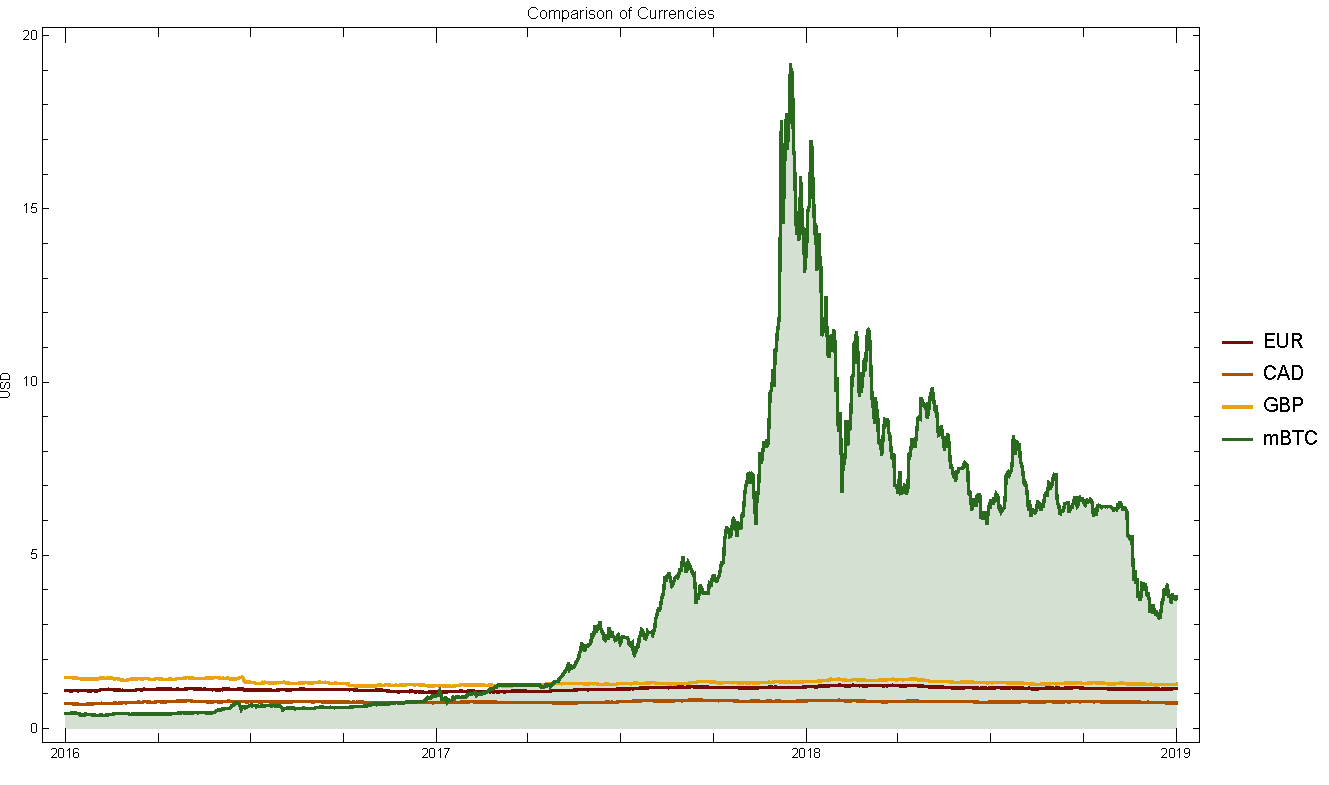
\includegraphics[width=0.8\textwidth]{figures/allCurrencies.pdf}
	\caption{\label{fig:btcandfiat}Comparison among fiat currencies and Bitcoin: The values are retrieved daily between  01 Jan 2016 and 01 Jan 2019. Note that 1000 mBTC = 1 BTC.}
\end{figure*}
%========================%

Without active management, the exchange rate of BTC with governmental currencies has been marked by extreme volatility (see Figure~\ref{fig:btcandfiat}). Squint at the chart to notice how the GBP drops around June 2016: this mild-looking pinch is actually the  `sharp decline' and `severe swing' that followed the Brexit referendum in the UK. However, it is completely overshadowed when placed beside BTC's large fluctuations.

\paragraph{A third wave?} Extreme volatility is not specific to Bitcoin (BTC), and can also be seen in its contemporaries Ethereum (ETH) and Ripple (XRP). This instability is an issue of practical importance: volatility encourages users to hoard (if it is going up) or avoid (if it is going down) the currency rather than use it. It makes lending risky, as currency movements can exceed interest payments. A lack of lending and credit inhibits the formation of mature financial markets. In response, a flood of proposals have been made for new cryptocurrency designs that purport to provide a stable exchange rate similar to (or exactly mirroring) a government-issued currency like the USD. These designs are called stablecoins.

Stablecoins have garnered a lot of attention recently, both positive and negative. According to \textit{CoinMarketCap}, more value in Tether changes hands across a given day than Bitcoin. This despite questions about Tether's reserves and regulatory investigations into its affiliates. The announcement of Facebook's Libra made international headlines and has been remarked on by the Fed, US legislators, and the even the sitting President. Another project, Basis (\nee Basecoin) raised \$133M in Venture Capital but folded up when it could not find a tenable path through US financial regulations. Central banks, including those of Sweden and Denmark, have explored the idea of government-issued stable cryptocurrencies.

\paragraph{Knowledge gap.} Understanding how stablecoins work should be easy. Most firms/projects have a whitepaper outlining the design, the coins are marketed to the general public, and there is no shortage of online articles surveying various designs. Unfortunately there are a number of pitfalls in systemizing this knowledge. Many whitepapers are obfuscated with jargon---terms left undefined and/or used inconsistently with other projects and with the financial literature. In other cases, system components appear to be mislabled. For example, a component that cleanly meets the definition of a security or a derivative might instead be labeled a bond or a loan. Maybe this is a lack of precision, or maybe it is a play to make an unconventional protocol appear more conventional? Or maybe they are unconscious attempts at keeping any regulatory red flags at half mast? In any case, we made a concentrated effort to offer direct and simple explanations (see Table~\ref{tab:mech}). In parallel to our work, other academics have produced their own taxonomies~\cite{PHP+19,MSS20}.

% = = = = = = = = = = = = = = = = = = = = = = = = = = = = = = = = 	
	
\begin{Sidebar*}[h!]
\begin{framed}
Sidebar
\begin{flushleft}
\textbf{Prices.} A cryptocurrency (like any asset) has two prices: (1) the most someone is willing to pay and (2) the least someone is willing to sell for. These are referred to as the best bid price and best offer (or ask) price respectively. Note that the best bid price should logically be less than the best offer price, otherwise an exchange would happen (such prices might occasionally `cross' but this should be temporal and quickly resolved with an exchange). Say a stablecoin is designed to ensure one unit is always priced at \$1 USD. To argue stability, one must show both that (1) the bid price should never exceed \$1 USD and (2) the offer price should never dip below \$1 USD. Note, conversely, that bids can dip below \$1 USD (everyone prefers to pay less than something is worth) and asks can exceed \$1 USD (everyone prefers to receive more than something is worth).
\end{flushleft}
\end{framed}
\end{Sidebar*}


% = = = = = = = = = = = = = = = = = = = = = = = = = = = = = = = = %

\begin{Sidebar*}[h!]
\begin{framed}
Sidebar
\begin{flushleft}
\textbf{Bitcoin \& Blockchain Primer.} A public blockchain is a type of distributed database (or ledger) that is open to anyone who wants to maintain it, robust against faulty and malicious participants, and runs without anyone in charge. When a participant looks at her local copy of the ledger, she is assured that (1) everyone has the exact same records and (2) each record was validated by the majority of participants before it was written into the ledger. Bitcoin is a digital currency that introduced the idea of a blockchain to track how much BTC is held by each account, and to write `smart' transactions for BTC payments. Transactions are added to the blockchain in a batch (called a block) by a network participant (called a miner) and miners include a special transaction that pays themselves newly minted BTC (called a coinbase transaction). The amount of new BTC released to miners follows a schedule built into the protocol and will decrement over time, eventually reaching zero once a determined amount of BTC has been made available. 
\end{flushleft}
\end{framed}
\end{Sidebar*}

% = = = = = = = = = = = = = = = = = = = = = = = = = = = = = = = = %

\begin{Sidebar*}[h!]
\begin{framed}
Sidebar
\begin{flushleft}
\textbf{Ethereum \& DApp Primer.} Ethereum is a blockchain protocol with a BTC-esque cryptocurrency called Ether (ETH). To a degree much greater than Bitcoin, Ethereum allows users to code verbose `smart contracts' or `decentralized apps (DApps)' that can be stored on the blockchain (for a fee). Once a DApp is deployed, users can run its functions (again, for a fee). The functions are executed by the miners and the output is written to the blockchain. Among other things, DApps can hold ETH and write functions that define how the ETH will be transferred from the DApp. DApps can also create their own currencies and circulate them as tokens. ERC20 tokens are compliant with a widely used Ethereum standard and can interoperate with existing wallet software, web-based exchanges, and token-tracking websites.
\end{flushleft}
\end{framed}
\end{Sidebar*}

% = = = = = = = = = = = = = = = = = = = = = = = = = = = = = = = = %


\section{How Do Stablecoins Work?}

We started by finding stablecoin projects on \textit{CoinDesk}, an online news source for cryptocurrencies, using search queries like ``stablecoins,'' ``stability,'' and ``price-stable.'' We read 185 articles up to January 11, 2019.\footnote{Given its high profile, we also include Facebook's Libra Coin which was released after this date.} For the 25 projects for which we could find sufficient documentation, we classified them in Table~\ref{tab:stablecoins}. This classification is done according to what the projects assert they do---we provide no warranty of what the projects do in reality. We sort projects according to their rank on \textit{CoinMarketCap} which ranks cryptocurrencies that are actively traded on an exchange service. Unlisted projects are ranked $\perp$.

Next, we distilled each proposal into a core stability mechanism. Instead of enumerating the intricate details of how each `brand' of stablecoin works---details that could change tomorrow---we concentrate on communicating the fundamentals. Broadly, the proposals can be split into two categories: (1) ones that try to directly match the stability of a second asset, such as the USD, and could not exist without this underlying asset, and (2) ones that propose independent currencies with algorithmic and/or human intervention mechanisms for providing stability. Fuller detail is provided in Table~\ref{tab:mech}.

% = = = = = = = = = = = = = = = = = = = = = = = = = = = = = = = = %

% !TEX root = ../main.tex

%-------------------Fancy Table ----------------------%

% = = = Rotated Table Entry \headrow


\newcommand{\headrow}[1]{\multicolumn{1}{c}{\adjustbox{angle=65,lap=\width-0.5em}{#1}}}

% = = = Table bullets: \full and \prt (full and part)

\newcommand{\full}{$\bullet$}
\newcommand{\prt}{$\circ$}

% ------------------------------------------------------------------------------------------------------------------------------------------------%
%Stablecoin projects%

\definecolor{UnitedNationBlue}{rgb}{0.30,0.53,1}
\definecolor{LightSteelBlue}{rgb}{0.69,0.77,0.87}
\definecolor{LightGrey}{rgb}{0.83,0.83,0.83}


\begin{table*}[t]
\centering

\begin{tabular}{|l|l|l|l|l|}

\hline
\rowcolor{lightgray}
\textbf{Class} & \textbf{Mechanism} & \textbf{Resembles} & Rank \\  \hline
% = = = = = = = = = = = = = = = = = = = = = = = = = = = = = = = = = = = = = = = = = = = = = = = = = = = = = = = = = = = = = = = = = = = = = = %
\multirow{17}{*}{Backed}		
						& \multirow{8}{*}{Directly-Backed \& Redeemable$^{\dagger}$}	& USDC 			& 20 \\ \cline{3-4}
						&													& TrueUSD 		& 26 \\ \cline{3-4}	
						&													& Paxos 			& 38 \\ \cline{3-4}		
						&													& Gemini Dollar 	& 52 \\ \cline{3-4}
						&													& StableUSD (USDS) & 685 \\ \cline{3-4}
						&													& Stronghold USD 	& 891 \\ \cline{3-4}
						&													& Petro 			& 1210 \\ \cline{3-4}
						&	& \multicolumn{1}{p{5cm}|}{Libra Coin, Ekon, WBTC, emparta} & $\perp$ \\ \cline{2-4}
% = = = = = = = = = = = = = = = = = = = = = = = = = = = = = = = = = = = = = = = = = = = = = = = = = = = = = = = = = = = = = = = = = = = = = = %
						& \multirow{6}{*}{Directly-Backed}  							& Tether 			& 6 \\ \cline{3-4}
						&													& EURSToken 		& 95 \\ \cline{3-4}
						&													& BitCNY 			& 304 \\ \cline{3-4}
						&													& Terracoin 		& 1280 \\ \cline{3-4}
						&													& Saga 			& 1495 \\  \cline{3-4}
						&	& \multicolumn{1}{p{5cm}|}{GJY, Novatti AUD, UPUSD} & $\perp$ \\ \cline{2-4} 						
% = = = = = = = = = = = = = = = = = = = = = = = = = = = = = = = = = = = = = = = = = = = = = = = = = = = = = = = = = = = = = = = = = = = = = = %
						& \multirow{3}{*}{Indirectly-Backed}							& Dai 			& 57 \\ \cline{3-4}
                                                &													& BitUSD 			& 398 \\  \cline{3-4}
                                                & 													& Nomin			& $\perp$ \\ \cline{1-4}
% = = = = = = = = = = = = = = = = = = = = = = = = = = = = = = = = = = = = = = = = = = = = = = = = = = = = = = = = = = = = = = = = = = = = = = %
%						& \multirow{1}{*}{Market Manipulation} 						& NuBits			& 892 \\ \cline{1-4}
\multirow{5}{*}{Intervention}                                                           

% = = = = = = = = = = = = = = = = = = = = = = = = = = = = = = = = = = = = = = = = = = = = = = = = = = = = = = = = = = = = = = = = = = = = = = %
						& \multirow{2}{*}{Money Supply Adjustments}  				& Ampleforth		& $\perp$  \\ \cline{3-4}
						&   													& RSCoin 			& $\perp$  \\ \cline{2-4}
% = = = = = = = = = = = = = = = = = = = = = = = = = = = = = = = = = = = = = = = = = = = = = = = = = = = = = = = = = = = = = = = = = = = = = = %
						& \multirow{2}{*}{Asset Transfer}  							& NuBits			& 892 \\ \cline{3-4}
						&													& CarbonUSD		& 1262 \\ \cline{3-4}
						&													& Basecoin 		& $\perp$ \\ \cline{1-4}
% = = = = = = = = = = = = = = = = = = = = = = = = = = = = = = = = = = = = = = = = = = = = = = = = = = = = = = = = = = = = = = = = = = = = = = %
%						& \multirow{2}{*}{TBD: Internal }  								& Nautiluscoin 		& $\perp$ \\ \cline{3-4}
% = = = = = = = = = = = = = = = = = = = = = = = = = = = = = = = = = = = = = = = = = = = = = = = = = = = = = = = = = = = = = = = = = = = = = = %
\hline
\end{tabular}
\caption{Stablecoin proposals as of January 11, 2019. $\dagger$ \textit{Disclaimer:} Projects are classified according to what they assert; \eg we provide no warranty that projects classified as `redeemable' provide actual redemption of the assets that back their coins. Rank corresponds to \textit{CoinMarketCap}.\label{tab:stablecoins}}
\end{table*}
% ------------------------------------------------------------------------------------------------------------------------------------------------%





% !TEX root = ../main.tex

\begin{table*}[t!]
\centering
\begin{tabular}{|l|}
\multicolumn{1}{c}{\textbf{Stability Mechanisms}}  \\ \hline

\multicolumn{1}{|p{\textwidth}|}{\textbf{Directly Backed and Redeemable.}\newline \footnotesize Alice is a trusted third party and uses Ethereum to instantiate a decentralized application (DApp) which issues 1000 AliceCoins as standard tokens (\eg ERC20). She asks \$1 USD for 1 AliceCoin and promises to redeem any AliceCoin for \$1 USD. If Bob buys 10 AliceCoins for \$10 USD, Alice deposits the \$10 USD in a bank account. Any time Alice receives a buy order for AliceCoins and does not have any left to sell, she creates new ones to sell. If Carol wants to redeem 5 AliceCoins, Alice withdraws \$5 USD and exchanges it with Carol, taking those AliceCoins out of circulation. Alice frequently publishes bank statements showing that her account holds enough USD to redeem all coins in circulation (the number of AliceCoins can be checked anytime on Ethereum).} \\ \hline

\multicolumn{1}{|p{\textwidth}|}{\textbf{Directly Backed.} \newline \footnotesize  Again, Alice is a trusted third party that issues 1000 AliceCoins as ERC20 tokens. She asks \$1 USD for 1 AliceCoin and promises to deposit and hold the payment in a bank account. As before, Alice creates new AliceCoins when she runs out and publishes frequent bank statements. Unlike above, she offers no direct redemption of AliceCoins for USD.} \\ \hline

\multicolumn{1}{|p{\textwidth}|}{\textbf{Indirectly Backed.} \newline \footnotesize Alice is no longer assumed to be trustworthy. She sets up a DApp that can hold ETH and issue tokens. The DApp determines how much ETH is equivalent to \$1.50 USD using the current exchange rate, provided to the DApp by a trusted third party oracle, and Alice deposits this amount of ETH into the DApp. The DApp issues to Alice two places in a line --- each place is a transferrable token. At some future time, the holder of the first place in line can redeem up to \$1.00 USD worth of the deposited ETH at the going exchange rate, and the holder of the second place in line gets any remaining ETH. Alice will transfer the first place in line (as a stable coin called AliceCoin) to Bob for \$1.00 USD, and will hold or sell the second place in line. When Bob redeems the AliceCoin, it will be worth \$1 USD in ETH when the entire deposit of ETH is worth more than \$1 USD. If the exchange rate drops enough, the entire deposit will be worth less than \$1 USD --- Bob will get all of the deposit and the holder of the second place in line will get nothing.} \\ \hline

\multicolumn{1}{|p{\textwidth}|}{\textbf{Money Supply Adjustments.} \newline \footnotesize Alice forks Bitcoin to create a new altcoin called AliceCoin. She tweaks the schedule for releasing new AliceCoins (called the coinbase amount in Bitcoin) according to the rules outlined below. She sets up a trusted oracle for the latest exchange rate of AliceCoins to USD. AliceCoin is programmed to apply an intervention when the price of an AliceCoin exceeds \$1.02 USD or dips below \$0.98 USD. If the price exceeds \$1.02 USD, the miner is allowed to increase the coinbase amount (the amount is determined by some mathematical relationship with how much the price exceeds \$1.02 USD). If the price dips under \$0.98 USD, the miner must decrease the coinbase amount based on the same relationship. The correctness of the claimed coinbase is verified by other miners in deciding to accept or reject a mined block, as per all other checked conditions in Bitcoin.} \\ \hline

\multicolumn{1}{|p{\textwidth}|}{\textbf{Asset Transfer.} \newline \footnotesize Alice instantiates a DApp with an ERC20 token called AliceCoin. The DApp is programmed to apply an intervention when the price of an AliceCoin exceeds \$1.02 USD or dips below \$0.98 USD according to a trusted oracle. If the price exceeds \$1.02 USD, the DApp creates new a set of AliceCoins (as above, according to some mathematical relationship) and transfers them to users waiting in line for them. How do users wait in line? When the price dips under \$0.98 USD, the DApp creates new positions at the end of the line and auctions them off to the highest bidder. The payment for a place in line is made in AliceCoins from the bidder to the DApp and the DApp destroys the payment. The place in line is a transferrable token. If the line is empty, AliceCoins are distributed according to a fallback policy (see main text).} \\ \hline

\end{tabular}
\caption{Major types of stability mechanisms for stablecoins.\label{tab:mech}}
\end{table*}


% !TEX root = ../main.tex

\begin{table}[t!]
\centering

	\begin{tabular}{ lllllllll}

&
\headrow{Corrects undervaluation} &
\headrow{Corrects overvaluation} &
\headrow{Decentralizes issuance } &
\headrow{Decentralizes redemption} &
\headrow{Decentralizes transfer} &
\headrow{No trusted oracle} \\
\hline

	 \multicolumn{1}{c}{\textit{Mechanism} } &    \multicolumn{2}{|c|}{Price} &  \multicolumn{4}{c}{Trust}  \\

	\hline

	Traditional Digital Cash			& \multicolumn{1}{|c|}{\full} & \multicolumn{1}{c|}{\full}   & \multicolumn{1}{c|}{} & \multicolumn{1}{c|}{} & \multicolumn{1}{c|}{} & \multicolumn{1}{c}{\full}   \\

	\hline

	Directly Backed and Redeemable	& \multicolumn{1}{|c|}{\full} 	& \multicolumn{1}{c|}{\full}   & \multicolumn{1}{c|}{} 		& \multicolumn{1}{c|}{} 		& \multicolumn{1}{c|}{\full} & \multicolumn{1}{c}{\full}    \\
	Directly Backed                              	& \multicolumn{1}{|c|}{} 		& \multicolumn{1}{c|}{\full}   & \multicolumn{1}{c|}{ } 	& \multicolumn{1}{c|}{} 		& \multicolumn{1}{c|}{\full} & \multicolumn{1}{c}{\full}    \\
	Indirectly Backed 				& \multicolumn{1}{|c|}{\prt} 	& \multicolumn{1}{c|}{\full}   & \multicolumn{1}{c|}{\full} 	& \multicolumn{1}{c|}{\full} 	& \multicolumn{1}{c|}{\full} & \multicolumn{1}{c}{}    \\      
%	Market Manipulation                       	& \multicolumn{1}{|c|}{\prt} 		& \multicolumn{1}{c|}{\prt}   & \multicolumn{1}{c|}{\full} 	& \multicolumn{1}{c|}{$\times$} 		& \multicolumn{1}{c|}{\full} & \multicolumn{1}{c}{}    \\ \hline
	Money Supply Adjustments             	& \multicolumn{1}{|c|}{?} 		& \multicolumn{1}{c|}{\prt}   & \multicolumn{1}{c|}{\full} 	& \multicolumn{1}{c|}{$\times$} 		& \multicolumn{1}{c|}{\full} & \multicolumn{1}{c}{}    \\
	Asset Transfer	                                & \multicolumn{1}{|c|}{?} 		& \multicolumn{1}{c|}{\prt}   & \multicolumn{1}{c|}{\full} 	& \multicolumn{1}{c|}{$\times$} 		& \multicolumn{1}{c|}{\full} & \multicolumn{1}{c}{}    \\
	\hline

	\end{tabular}
	\caption{Comparative evaluation of mechanisms to design stablecoins: {\full} indicates the properties (columns) are fulfilled by the corresponding mechanism (rows) within reason, {\prt} means the property is fulfilled but the fulfillment is bounded, {?} indicates a heuristic has been proposed for stability and the conditions under which it will work are not well-established enough to evaluate, and $\times$ indicates the property is not applicable.
	\label{tab:evframework}}
\end{table}

% = = = = = = = = = = = = = = = = = = = = = = = = = = = = = = = = %

\section{Type 1: Backed Stablecoins}
\label{sec:t1}

\subsection{Directly-Backed and Redeemable}
\label{sec:redeem}

For stablecoins in this category, the firm operating the currency will obtain a reserve of some valuable asset---it might be USD or another sovereign currency, gold or another commodity, or a basket of multiple assets.  It will then issue digital tokens that represent a unit of the underlying asset (to illustrate, assume a token is redeemable for 1 USD) which can be exchanged online.

This idea predates Bitcoin: Liberty Reserve provided a similar digital currency, with some caveats about its redeemability (not to mention its legality). However Liberty Reserve, e-gold, and similar pre-blockchain services would maintain transaction details and account balances on a private server. Blockchain enables decentralized trust for the transactions, while the coin creation and redemption processes rely on a trustworthy firm. In short, this type of stablecoin is more centralized than Bitcoin but less than Liberty Reserve. For analysis, we need a finer grained approach to trust assumptions which Table~\ref{tab:evframework} tries to capture. Also consider that while decreasing centralization can be good for trust and transparency, additional measures are needed to ensure it is not harmful for privacy.

Recall the mechanism for issuing AliceCoins in Table~\ref{tab:mech}. If buyers are willing to pay more than \$1 USD for 1 AliceCoin, new coins can be generated for \$1 USD and sold to these buyers for a profit, ensuring bids return to \$1 USD (it corrects overvaluation). If sellers are willing to take less than \$1 USD for 1 AliceCoin, these coins can be bought and redeemed for a profit, ensuring offers return to \$1 USD (it corrects undervaluation). In reality, transactions are not free, efficient, or entirely frictionless and some price deviation is expected. If redemption is ever in doubt, then the price can fall freely from \$1 USD (although this will not necessary happen, see next section). The trustworthiness of the operating firm and the custodian of the reserves is essential, and financial audits are an important step to establishing confidence (although many pitfalls exist when auditing blockchain-based assets~\cite{PBEC19}). 

% = = = = = = = = = = = = = = = = = = = = = = = = = = = = = = = = %

\subsection{Directly-Backed}
\label{sec:tether}

What if a stablecoin operated exactly as in the previous section but did not offer a redemption process for the coin's underlying assets? If we could not find a clear assertion of redemption, we listed the project under this category in Table~\ref{tab:stablecoins}.

Recall the mechanism in Table~\ref{tab:mech}. Bids will not exceed \$1 for the same reason as the previous section. However there is no longer a way to profit if offers vary between \$0 USD to \$1 USD (\ie the mechanism does not prevent undervaluation). Generally coins in this category are in fact `redeemable' by one user: the firm operating the coin. It could purchase undervalued coins to release \$1 USD from its reserves. For this reason, stablecoins in this category are scrutinized (to the extent made possible by the firm) to ensure reserves are intact. If every AliceCoin was not backed by \$1 USD, Alice could overissue AliceCoins to enrich herself.

The largest coin is this category is Tether. Tether claims to be redeemable, but the redemption process is reported by users to have a lot of friction, it is accused of issuing coins to manipulate markets~\cite{griffin2018bitcoin}, and it has not always maintained full reserves of USD to allow all Tether to be redeemed (for these reasons, we categorize it here). To many, it is a mystery why Tether remains highly liquid with daily trading volumes exceeding all other cryptocurrencies in value (according to \textit{CoinMarketCap} at the time of writing). One explanation is that it is too useful to fail.

A key use-case, illustrated by Tether and the affiliated exchange Bitfinex, is as a temporary store of value for traders and speculators. A trader that wants to divest their BTC for USD has three options. She can (1) hold the USD in her exchange account, which can be used only on the same exchange and requires the exchange to be a trustworthy custodian. She can (2) withdraw the USD from the exchange but this requires identity verification (in most jurisdictions), a bank that will accept proceeds of cryptocurrency trading, and a substantial time delay. A balanced alternative is to (3) exchange BTC into a stablecoin which can be withdrawn from the exchange (\ie moved from the exchange to Alice's private key) with little friction, delay, or regulatory oversight. The withdrawn stablecoin can be moved onto a different exchange, transferred to other users, or used for direct purchases without involving the original exchange. In short, it offers more flexibility than leaving USD in an exchange account and less friction than withdrawing USD.
 
% The idea of tokenizing assets and re-selling them in a useful format (\eg as a portfolio or in a way that is digitally compliant with standard trading software and automated accounting systems) is commonplace for standard financial assets, however most tokenizations of this type have some direct or indirect redeemable value. Consider two contrasting examples: a typical ETF and a typical trust fund. An electronically traded fund (ETF) will typically sell shares of a portfolio of assets, be redeemable for the assets on-demand, and will be priced closely ($\pm 1\%$) to the value of its underlying assets---it is most like the stablecoins in Section~\ref{sec:redeem}. A simplification of a (close-ended) trust fund is as follows: a firm will set up a special corporation to hold the assets, the tokens are not directly redeemable, however the tokens are ownership shares in the special corporation---by owning the corporation, you effectively own its assets. Such a fund will trade with greater deviation from the value of its assets ($\pm 5\%$).

% A coin that has no redemption, direct or indirect, will not clearly be traded for a particular amount. An informal argument in favour of it being stable is that minting the coin is costly---it requires obtaining USD to hold in reserve. This feature serves an important function, albeit a different one. This bounds the firm from over-issuing tokens, which would cause the coin to lose value, however it does not ensure asks do not drop below \$1 USD.

% The difference between the market value of a newly minted coin and the cost to produce it is called seignorage. A backed stablecoin has no seignorage: it sells for \$1 USD and requires holding \$1 USD to `produce' it. There appears to be a folk theorem that if minting asset X requires consuming asset Y, asset X will take on the value of asset Y (otherwise, who would produce X?). In reality, resources can be consumed to produce something of no value---that value is simply lost. A canvas that has been applied with acrylic paint might cost \$100 USD in raw materials; its value could none-the-less be much less than \$100 USD\ldots or much more.

% If Alice goes to Peter Luger's in Brooklyn, consumes a \$100 ribeye, and mints a literal shitcoin out of the result --- is that coin worth \$100 because it is ``backed'' by \$100 worth of steak?

% = = = = = = = = = = = = = = = = = = = = = = = = = = = = = = = = %

\subsection{Indirectly-Backed}
\label{sec:dai}

Both of the previous mechanisms placed heavy trust assumptions on the firm operating the currency. Could a currency be managed autonomously by a DApp? The key idea of this mechanism is to offer a redeemable token that can be converted into \$1 USD worth of ETH at the going USD/ETH exchange rate. Therefore the amount of ETH received ETH will grow or shrink depending on the exchange rate. Because a blockchain has no inherent knowledge of exchange rates, this mechanism still requires one trustworthy entity called an oracle to write the exchange rate into the blockchain (or consensus can be taken across a set of oracles).

Recall the mechanism in Table~\ref{tab:mech}. Bids for an AliceCoin in excess of \$1 USD will be fulfilled as long as there are individuals like Alice willing to lock up a deposit of ETH that is $1.5\times$ the face-value of what they receive (this is called over-collateralization). An AliceCoin offered for less than \$1 USD can be purchased and redeemed for a profit--assuming the DApp holds enough ETH. Otherwise, an AliceCoin will sell between \$0 and \$1 USD according to the value of the ETH held by the DApp. 

Is it risky for Alice to offer such an AliceCoin? Holding the second place in line is more volatile than holding ETH itself---this stability mechanism does not (and cannot) eliminate volatility, it simply pushes it from the first place to the second place in line. However the second place in line is never more than \$1 USD short of the full amount of ETH held in the DApp. So if Alice keeps the \$1 USD she received for the AliceCoin, it offsets any losses from the second place in line. She has no more risk than holding ETH. The second place in line can also be sold to someone who is seeking risk: the token is a leveraged bet that ETH rises in value. Is it risky for Bob? In most conditions, holding an AliceCoin is purposefully the same as holding USD. However if the USD/ETH rate deteriorates quickly, the AliceCoin will use up its buffer and start to lose value (at the same rate as ETH).

Here are just a few of the design decisions to consider when deploying an indirectly-backed stablecoin: what should the overcollateralization ratio be (\eg 1.5x)? When can an AliceCoin be redeemed (\eg on-demand, after an elapsed time, after movements in USD/ETH, \etc)? How do you issue multiple AliceCoins (\eg collateral for each coin is held separately, or collateral for all coins are pooled together and coins are interchangeable)?

% This stability mechanism might enable a third-party to trigger a redemption (\eg for a fee) if they notice a deposit is close to losing more value than the face value of the coins (before the coin holder does). Note that while allowing third parties to trigger a redemption seems like a sensible service, if the coin holders are not monitoring the situation, they will end up holding ETH, instead of an AliceCoin, which is still losing value. Thus this mechanism does not protect holders of the stablecoin at all --- it is really only about maintaining the reputation of the stablecoin. The stablecoin can claim it has never broken its peg to the dollar but it is an illusion, because as soon as it is about to lose value, it turns back into its collateral and then loses values under the name of the collateral instead of the stablecoin. If the holder isn't paying attention, they actually lose more by having it triggered than they would breaking the buck.

% Use this for stocks? 

% = = = = = = = = = = = = = = = = = = = = = = = = = = = = = = = = %

\section{Type 2: Intervention-based Stablecoins}
\label{sec:t2}

% Intervention-based
% Input is exchange rate -> exchange rate reigme which has failed (see CBDC paper)
% Hard to see what else could be used

%Instead, most stablecoin projects use the exchange rate with a fiat currency (\eg the USD) as input to the intervention mechanism. This makes these coins look more similar to coins that are backed by USD (in Section~\ref{sec:t2}). This is good for cross-comparison in a paper like this, but the reader should bear in mind that any economic metric could be used instead with these coins, including ones not based on an exchange rate. Second, we remark that central banks in the past have used exchange rates to decide when to intervene, but this approach was not found inadequate for stablising an economy. Alternatives to the exchange rate might include interest rates (if lending markets emerge), purchasing power, or measurements on the amount, volume, and/or velocity of transactions. The challenge for these is ensuring the metrics cannot be easily manipulated in the blockchain environment, where single entities can create unlimited identities and wash transactions, trades, loans, \etc with themselves. If the metric(s) could be inferred from the blockchain itself, the stability mechanism could be autonomous and fully decentralized. 

% Supply-side changes

%The second design decision is what intervention to make. All the stablecoin projects in this category make the same fundamental intervention: the supply of the stablecoin is increased to curb the value of the currency, and the supply is contracted to boost its value. The final design decision is how exactly the supply is manipulated. Some coins very directly influence the money supply, while other coins try to turn currency into assets to contract, and turn assets into currency to expand. This is obviously inspired by how modern central banks influence interest rates.\footnote{Central banks will purchase assets, like government bonds, from banks at competitive prices to increase the bank's cash and lower the interest rate at which the bank will lend. Conversely, they will sell assets to the banks at competitive prices to remove cash from the banks, causing a greater demand for cash loans, which tends to increase inter-bank interest rates.} The final design decision is deciding who participates in these mechanisms. 

% Heuristics

% In this section, we refer to the proposed stability mechanisms as \textit{heuristics} because their validity can only be shown within models that may or may not actually model human (and trader) behaviour. In fact, this is the best case scenario. Most of these heuristics do not even have models or simulations showing the conditions under which they work, however there is interesting future work to be done here. 

% We cannot prove that something here works or not. It is all heuristics. We know this because central banks themselves operate on heuristics that change every couple of decades. Even if we cannot say something does work, we can point out a few suggestions that it will not work. Game-able inputs, inputs/interventions that have not worked for currency.
 
% = = = = = = = = = = = = = = = = = = = = = = = = = = = = = = = = %

\subsection{Money Supply Adjustments}
\label{sec:elastic}

A trusted oracle provides the going exchange rate between the cryptocurrency and a stable-valued asset, such as the USD. When the cryptocurrency gains value, the supply of the cryptocurrency is increased, and when it loses value, the supply is decreased. This mechanism is based on how central banks have historically controlled their economies, however the specifics of exchange rate targetting have been abandoned by modern central banks after past failures. That said, exchange rates are an illustrative example and other financial indicators could be used: oracle-provided interest rates (should lending markets emerge) or purchasing power; on-blockchain metrics like transaction volumes (should these prove robust against manipulation), or human discretion (such as central banks themselves~\cite{danezis2015centrally}).

Allowing a crypto-currency to expand is not difficult. Who receives the new currency is a design decision with options including: (1) existing holders of the currency in proportion to their holdings, (2) existing holders through a random lottery, (3) miners, or (4) a specific entity like a central bank. Who loses when the currency contracts is the primary challenge.

The mechanism in Table~\ref{tab:mech} gives one illustration. Here if many bids for AliceCoin exceed \$1.02 USD, some of the newly injected currency could be spent on obtaining USD until all buyers willing to pay more than \$1.02 USD have purchased AliceCoins. This is merely a heuristical argument because there is no guarantee the recipients will spend the new currency on USD, especially if demand for USD is falling. The justification for offers below \$0.98 is symmetric: the currency contractions could make holders less willing to spend it on USD. However if the price drop is caused by a lack of demand for AliceCoins rather than an oversupply, then removing supply will only thin out the market but not actually incentivize traders to trade and correct the undervaluation.

When the coinbase is increased or decreased dynamically (called an elastic coinbase), increases can be by any amount but decreases cannot appear to go past zero. When the coinbase is exactly zero, miners are still incentivized to mine because of the fees provided in the transactions. In fact this is how Bitcoin will eventually (projected to happen in 2140) function once all BTC is created (how well it will work is debatable~\cite{carlsten2016instability}). Could the coinbase go negative? Since miners are rewarded the sum of the coinbase and the transaction fees, a coinbase can indeed be moderately negative if the transaction fees are greater than the negative coinbase. Under this deployment, the users are effectively burning their transaction fees to contract the money supply.


\subsection{Asset Transfer}
\label{sec:basecoin}

The second subtype of intervention-based stability mechanism expands and contracts the supply of currency to influence its value, however it uses a less direct contraction method. Recall the mechanism in Table~\ref{tab:mech}. If many bids in excess of \$1.02 USD remain unexecuted, the logic follows the previous section: the currency is handed out in hopes that more USD will be bought. The justification for offers below \$0.98 is premised on individuals buying places in line, and if this premise is true, the resulting contraction of the currency follows the same logic as the previous section. The purchase of a spot in line is highly speculative --- the currency might not return to stability and the spot might never be reached. As the line gets longer, the price of a place in line will fall, and the speculative market will thin out to traders wanting a higher and higher risk/reward ratio. These trends do not guarantee, or even point toward, a recovery in price. 

% = = = = = = = = = = = = = = = = = = = = = = = = = = = = = = = = %

%========================%
\begin{figure*}[t]
	\centering
	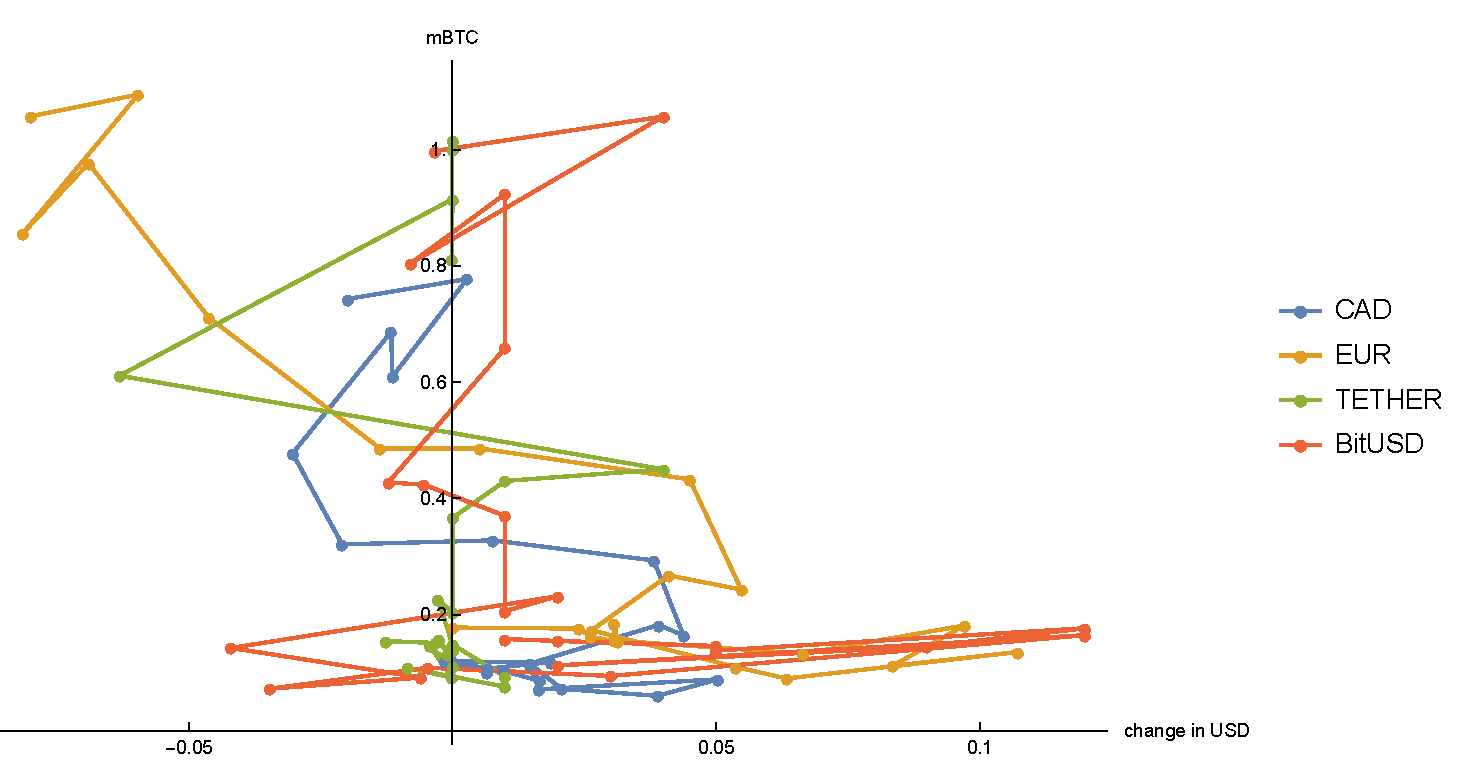
\includegraphics[width=0.8\textwidth]{figures/newGraph.pdf}
	\caption{\label{fig:vol}
	Volatility in prices for two fiat currencies (CAD and EUR) and two stablecoins (Tether and BitUSD) against the USD and BTC.
	Vertical line segments demonstrate USD stability. 
	Horizontal show the currency tracking BTC.
	For further interpretation, see~\cite{CDM19}.
	While CAD and EUR are not pegged to USD, they demonstrate a degree of stability not that different from the stablecoins. 
	Prices from Jan 2017 to Nov 2018; 1000 mBTC = 1 BTC.}
\end{figure*}
%========================%

\section{Discussion and Conclusion.}

A more detailed version of this article is available as a whitepaper~\cite{CDM19}. It includes more detail about each coin, some empirical studies of how stable these coins are (see Figure~\ref{fig:vol} for a preview), and an evaluation of whether of Ethereum's mechanism for paying for computation (gas) is stable or not (the answer: it does not seem to be, for now).

In short, stablecoins might tokenize a low volatility coin and bring it onto the blockchain. Or they generally play one of two tricks. The first trick is to expand and contract the amount of currency to stabilize the value. The second trick is to turn two high volatility coins (\eg of the underlying cryptocurrency) into one stablecoin and one extremely volatile coin. This last trick is similar to other financial assets which do not reduce overall risk, but instead push it from one tranche of the asset to another.

Why are there so many projects? The differentiation between coins is along a few parameters: (1) the type of asset that can be redeemed for the coin: USD, EUR, gold, \etc; (2) the underlying blockchain (\eg Bitcoin, Ethereum, \etc) and the low-level technical design (updatable contracts, governance, \etc); and (3) the country it operates from which determines the degree of regulatory compliance that's required. 

What's next? Self-sovereign stablecoins are interesting and probably here to stay, however they face numerous regulatory hurdles from banking, financial tracking, and (likely) securities laws. For stablecoins backed by a governmental currency, the ultimate expression would be a centrally banked digital currency (CBDC). Since paper currency has been in steady decline (and disproportionately for legitimate transactions~\cite{rogoff2017curse}), a CBDC could reintroduce cash with technological advantages and efficient settlement while minimizing user fees.

\begin{acks}

J. Clark acknowledges support for this research project from the \grantsponsor{A19}{Autorit\'e des March\'es Financiers (AMF)}{https://lautorite.qc.ca/en/general-public/about-the-amf/amf-strategic-financial-education-outreach-and-research-partnerships-program/} and from the \grantsponsor{N19}{NSERC/RCGT/Catallaxy Industrial Research Chair in Blockchain Technologies}{https://www.nserc-crsng.gc.ca/Chairholders-TitulairesDeChaire/Chairholder-Titulaire_eng.asp?pid=1045}. S. Moosavi acknowledges support from \grantsponsor{F19}{The Fonds de recherche du Québec - Nature et technologies (FRQNT)}{http://www.frqnt.gouv.qc.ca/en/accueil}.


\end{acks}










